\documentclass{article}
%\usepackage{custom}
\usepackage{amsmath, amsfonts, amsthm, amssymb}
\usepackage{fancyvrb}
\usepackage{relsize}
\usepackage{tikz}
\usetikzlibrary{shapes,backgrounds}

\RecustomVerbatimEnvironment
  {verbatim}{Verbatim}
  {fontfamily=courier,fontsize=\relsize{-2},frame=single}

\pagestyle{myheadings}
\markboth{Venn Diagrams by H. Duong}{Venn Diagrams by H. Duong}

\begin{document}

\section*{Introduction}

One way to create Venn diagrams is through a packaged called
\verb|tikz|. For ease of use, we also use \verb|\usetikzlibrary{shapes,backgrounds}| which is a command within
\verb|tikz| that provides shortcuts for certain shapes and colors.
A typical \LaTeX\ document would have the following header:
\begin{verbatim}
\documentclass{article}
\usepackage{custom}
\usepackage{tikz}
\usetikzlibrary{shapes,backgrounds}
\end{verbatim}
Note that \verb|\usetikzlibrary| must come after 
\verb|\usepackage{tikz}|
because that command is only available after we specify the use of the \verb|tikz| package.

\section*{Simple Examples}

Within the document body, we can specify a \verb|tikz| graphic
object using the \verb|tikzpicture| environment. The following
code
\begin{verbatim}
\begin{center}
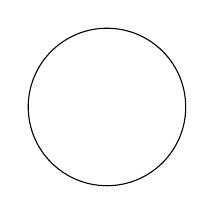
\begin{tikzpicture}
	\draw (0,0) circle (1cm);
\end{tikzpicture}
\end{center}
\end{verbatim}
would produce a circle as shown below. The circle is centered at
the point $(0,0)$ and has a radius of 1cm. The center is actually located at $(0\text{cm}, 0\text{cm})$. That is, if
no units are specified, then centimeters is the default unit
of measure.
\begin{center}
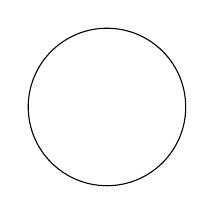
\begin{tikzpicture}
	\draw (0,0) circle (1cm);
\end{tikzpicture}
\end{center}

It is possible to make other shapes such as arcs, ellipses, and
rectangles, to name a few. For Venn diagrams, we only need
the syntax for circles and rectangles. The code below shows
both cases in a single graphic object. Rectangles are specified by their corners. 
\begin{verbatim}
\begin{center}
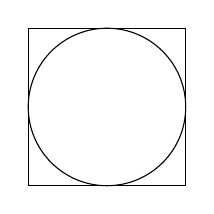
\begin{tikzpicture}
	\draw (0,0) circle (1cm);
	\draw (-1,-1) rectangle (1,1);
\end{tikzpicture}
\end{center}
\end{verbatim}
\begin{center}
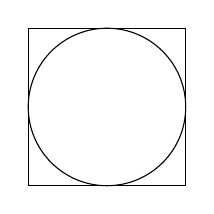
\begin{tikzpicture}
	\draw (0,0) circle (1cm);
	\draw (-1,-1) rectangle (1,1);
\end{tikzpicture}
\end{center}

\section*{Shading}

To shade in regions, we use the \verb|\fill| command. 
\begin{verbatim}
\begin{center}
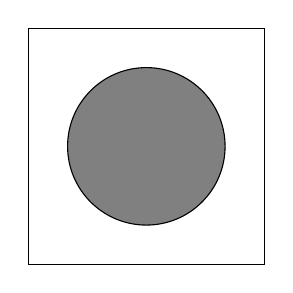
\begin{tikzpicture}
	\fill[gray] (0,0) circle (1cm);
	\draw (0,0) circle (1cm);
	\draw (-1.5,-1.5) rectangle (1.5,1.5);
\end{tikzpicture}
\end{center}
\end{verbatim}
\begin{center}
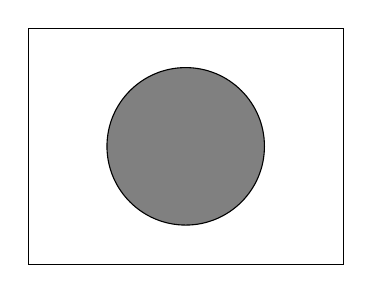
\begin{tikzpicture}
	\fill[gray] (0,0) circle (1cm);
	\draw (0,0) circle (1cm);
	\draw (-2,-1.5) rectangle (2,1.5);
\end{tikzpicture}
\end{center}
The order in which the commands appear is important. The
first command fills in a circular region cetered at $(0,0)$
and having radius 1cm. The second command then draws a
circle with the same properties. Without the second line,
we would only see a gray circular region, but not the darker
outline on the boundary of the circle.


\section*{Command Order}

Consider the following code and its corresponding diagram.
\begin{verbatim}
\begin{center}
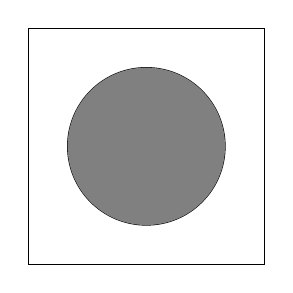
\begin{tikzpicture}
	\draw (0,0) circle (1cm);
	\fill[gray] (0,0) circle (1cm);
	\draw (-1.5,-1.5) rectangle (1.5,1.5);
\end{tikzpicture}
\end{center}
\end{verbatim}
\begin{center}
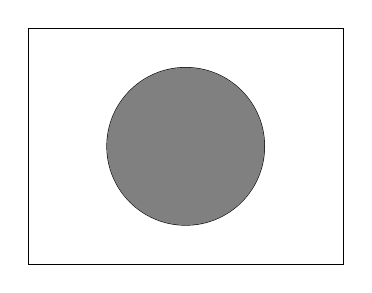
\begin{tikzpicture}
	\draw (0,0) circle (1cm);
	\fill[gray] (0,0) circle (1cm);
	\draw (-2,-1.5) rectangle (2,1.5);
\end{tikzpicture}
\end{center}
Since the fill command appears {\bf after} the draw command, we no longer see a dark outline on the boundary of the circular region. The reason is that the circle created
by the draw command is covered by the gray color
in the fill command. So if a command that appears later
happens to draw over the same area that contains objects
from previous commands, then those previously visible objects
are covered by the most recently created object. Below is
an series of diagrams that depicts what happens in sequence.

\begin{verbatim}
\begin{center}
\begin{tikzpicture}
	\draw (-2,-1.5) rectangle (3,1.5);  % draw only a rectangle
\end{tikzpicture}
\end{center}
\end{verbatim}
\begin{center}
\begin{tikzpicture}
	\draw (-2,-1.5) rectangle (3,1.5);
\end{tikzpicture}
\end{center}


\begin{verbatim}
\begin{center}
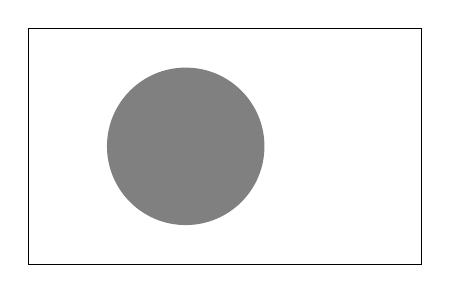
\begin{tikzpicture}
	\draw (-2,-1.5) rectangle (3,1.5);  % draw a rectangle
	\fill[gray] (0,0) circle (1cm);     % then fill in a circular region
\end{tikzpicture}
\end{center}
\end{verbatim}
\begin{center}
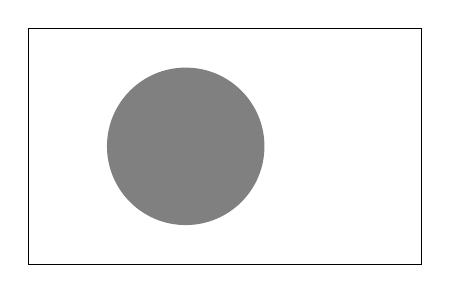
\begin{tikzpicture}
	\draw (-2,-1.5) rectangle (3,1.5);
	\fill[gray] (0,0) circle (1cm);
\end{tikzpicture}
\end{center}

\begin{verbatim}
\begin{center}
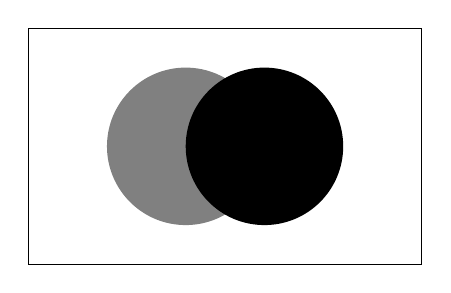
\begin{tikzpicture}
	\draw (-2,-1.5) rectangle (3,1.5);  % draw a rectangle
	\fill[gray] (0,0) circle (1cm);     % then fill in a circular region
	\fill[black] (1,0) circle (1cm);    % then fill in a 2nd circular region
\end{tikzpicture}
\end{center}
\end{verbatim}
\begin{center}
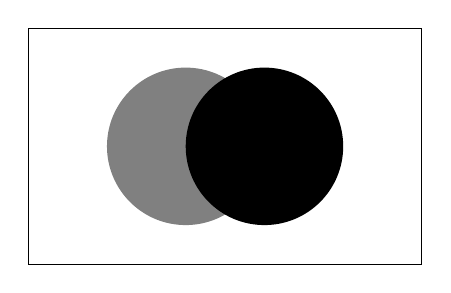
\begin{tikzpicture}
	\draw (-2,-1.5) rectangle (3,1.5);
	\fill[gray] (0,0) circle (1cm);
	\fill[black] (1,0) circle (1cm);
\end{tikzpicture}
\end{center}


\section*{Nodes}

Every object within a \verb|tikz| picture
is associated with a point,
or many points. For example, a circle is defined by a point 
(its center) and its radius. A rectangle is associated with
two (corner) points. Lines can be drawn via their two endpoints.
A node, then, is simply the most recently referenced point.
It is usually used to designate a location, such as where
to place a label. Below is an example of how to label a diagram using nodes.
\begin{verbatim}
\begin{center}
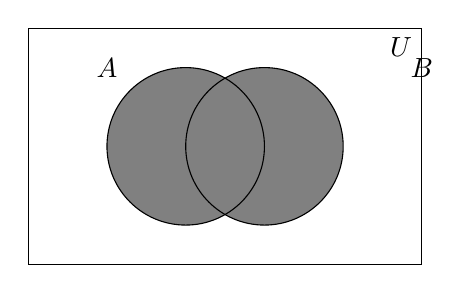
\begin{tikzpicture}
	\draw (-2,-1.5) rectangle (3,1.5) node[below left]{$U$}; 
	\fill[gray] (0,0) circle (1cm);
	\fill[gray] (1,0) circle (1cm);
	\draw (0,0) circle (1cm);
	\draw (1,0) circle (1cm);
	\draw (-1,1) node {$A$};
	\draw (3,1) node {$B$};
\end{tikzpicture}
\end{center}
\end{verbatim}
\begin{center}
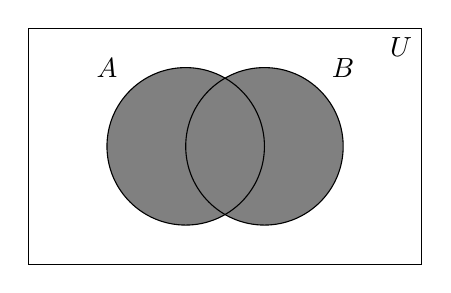
\begin{tikzpicture}
	\draw (-2,-1.5) rectangle (3,1.5) node[below left]{$U$}; 
	\fill[gray] (0,0) circle (1cm);
	\fill[gray] (1,0) circle (1cm);
	\draw (0,0) circle (1cm);
	\draw (1,0) circle (1cm);
	\draw (-1,1) node {$A$};
	\draw (2,1) node {$B$};
\end{tikzpicture}
\end{center}
We could have labeled the two circles using their centers as well.
\begin{verbatim}
\begin{center}
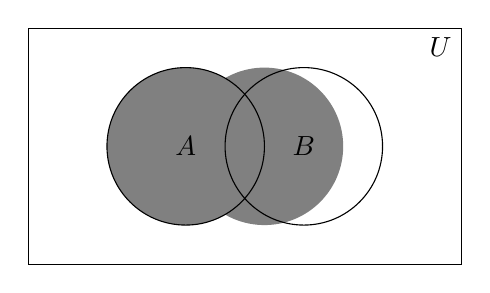
\begin{tikzpicture}
	\draw (-2,-1.5) rectangle (3.5,1.5) node[below left]{$U$}; 
	\fill[gray] (0,0) circle (1cm);
	\fill[gray] (1,0) circle (1cm);
	\draw (0,0) circle (1cm) node {$A$};
	\draw (1.5,0) circle (1cm) node {$B$};
\end{tikzpicture}
\end{center}
\end{verbatim}
\begin{center}
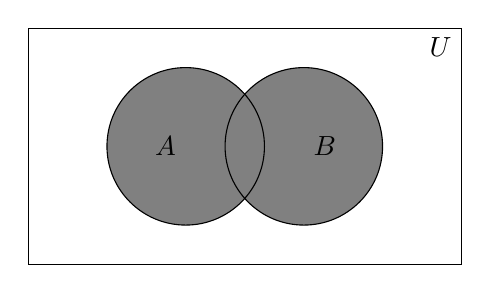
\begin{tikzpicture}
	\draw (-2,-1.5) rectangle (3.5,1.5) node[below left]{$U$}; 
	\fill[gray] (0,0) circle (1cm);
	\fill[gray] (1.5,0) circle (1cm);
	\draw (0,0) circle (1cm) node[left] {$A$};
	\draw (1.5,0) circle (1cm) node[right] {$B$};
\end{tikzpicture}
\end{center}
In the example above, we made the centers of the two circles
slightly further apart. Notice the slight reduction in code
since the nodes are using the previously referenced centers
of each circle as their location as opposed to having to
specify the actual locations of the nodes in the previous
example.

\section*{Clipping}

There are certain regions which we wish to shade in a Venn
diagram that do not correspond to any basic geometrical object.
While it is easy to create a Venn diagram for $A\cup B$ (see
previous example), creating a Venn diagram for $A\cap B$
requires the use of clipping.

``Newspaper clippings'' is a common use of the word clipping,
and its meaning in computer graphics is similar to that of
newspaper clippings. When we make a newspaper clipping, we cut
out portions of the newspaper which we wish to keep. The idea
is the same with graphics clippings. To create a Venn diagram
for $A\cap B$, we can think of the result as ``clipping out
$A$ from $B$'' in the sense that $B$ is the newspaper, and only
the portions within $A$ that are in the newspaper $B$ are
kept. Here is what the code and diagram looks like.
\begin{verbatim}
\begin{center}

\begin{tikzpicture}
	\clip (0,0) circle (1cm);           % keep only what is inside A
	\fill[gray] (1.5,0) circle (1cm);   % draw B region
\end{tikzpicture}
\end{center}
\end{verbatim}
\begin{center}

\begin{tikzpicture}
	\clip (0,0) circle (1cm);           % keep only what is inside A
	\fill[gray] (1.5,0) circle (1cm);   % draw B region
\end{tikzpicture}
\end{center}

Now put in all the other elements such as the universal set $U$
and some labels for the two subsets $A$ and $B$. Unfortunately,
if we use:
\begin{verbatim}
\begin{center}
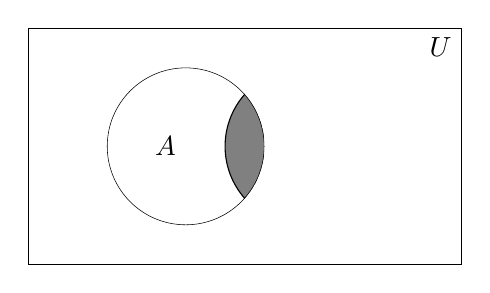
\begin{tikzpicture}
	\draw (-2,-1.5) rectangle (3.5,1.5) node[below left]{$U$}; 
	\clip (0,0) circle (1cm);           % keep only what is inside A
	\fill[gray] (1.5,0) circle (1cm);   % draw B region
	\draw (0,0) circle (1cm) node[left] {$A$};
	\draw (1.5,0) circle (1cm) node[right] {$B$};
\end{tikzpicture}
\end{center}
\end{verbatim}
we obtain what may initially appear to be unexpected results:
\begin{center}
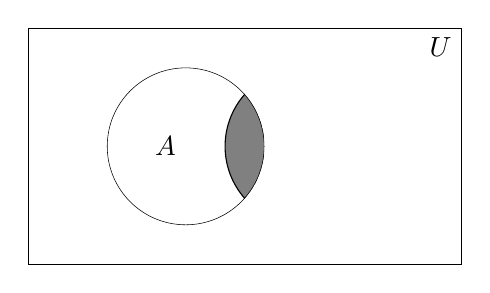
\begin{tikzpicture}
	\draw (-2,-1.5) rectangle (3.5,1.5) node[below left]{$U$}; 
	\clip (0,0) circle (1cm);           % keep only what is inside A
	\fill[gray] (1.5,0) circle (1cm);   % draw B region
	\draw (0,0) circle (1cm) node[left] {$A$};
	\draw (1.5,0) circle (1cm) node[right] {$B$};
\end{tikzpicture}
\end{center}
The next section explains another caveat that is closely linked
with the fact that commands are recognized in the order that
they appear.

\section*{Scope}

In the last example, it should be clear that everything drawn 
{\bf after} the \verb|\clip| command will only be visible
{\bf if the object happens to reside inside the circle $A$}.
So the clip command is more like a filter that only allows
objects whose parts lie within circle $A$ to be drawn! (We
can use any valid \verb|tikz| shape, of course.)
How can we limit the scope of such a command? Below is
an example of how the scope environment limits what exactly
does  get clipped.

\begin{verbatim}
\begin{center}
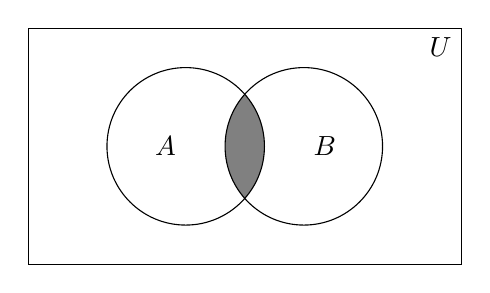
\begin{tikzpicture}
	\draw (-2,-1.5) rectangle (3.5,1.5) node[below left]{$U$}; 
	\begin{scope}                       % start of clip scope
	\clip (0,0) circle (1cm);
	\fill[gray] (1.5,0) circle (1cm);
	\end{scope}                         % end of clip scope
	\draw (0,0) circle (1cm) node[left] {$A$};
	\draw (1.5,0) circle (1cm) node[right] {$B$};
\end{tikzpicture}
\end{center}
\end{verbatim}

\begin{center}
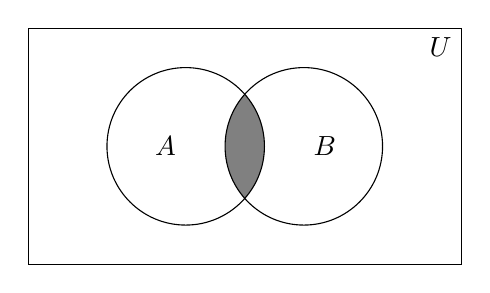
\begin{tikzpicture}
	\draw (-2,-1.5) rectangle (3.5,1.5) node[below left]{$U$}; 
	\begin{scope}
	\clip (0,0) circle (1cm);           % keep only what is inside A
	\fill[gray] (1.5,0) circle (1cm);   % draw B region
	\end{scope}
	\draw (0,0) circle (1cm) node[left] {$A$};
	\draw (1.5,0) circle (1cm) node[right] {$B$};
\end{tikzpicture}
\end{center}


\section*{Alternate Syntax for Points}

A slightly different means of specifying a point is to use
the format $(\theta : r)$ where $\theta$ is an angle in 
degrees and $r$ is the distance from the origin. So for
example, the point $(3,4)$ is the same as $(53.13 : 5)$
since $\arctan(4/3) \approx 53.13^\circ$ and 
$5=\sqrt{3^2+4^2}$.\

 An example of where this would be useful
is if we wish to have three sets (represented as circles)
that are ``evenly spaced'' in our Venn diagram. If two
of them have centers at $(0,0)$ and $(1.5,0)$, then a
natural choice for the third center is a point $(x,y)$ such
that $(0,0)$, $(1.5,0)$, and $(x,y)$ form an equilateral
triangle. So rather than spending time computing the
proper values of $(x,y)$, we could just use $(60 : 1.5)$
since the triangle would have to have three $60^\circ$ 
angles and each side would be of length 1.5. We will demonstrate such an example later.

\section*{Simplifying Everything}

One last thing to consider is how we could reduce the amount
of code we need to type to generate these diagrams. Notice
that all our circles had a radius of 1cm. We can create
shortcuts for ``\verb|(0,0) circle (1cm)|'' using
\begin{verbatim}
\def \setA{ (0,0) circle (1cm) }
\end{verbatim}
and then use \verb|\setA| instead. For example,
\begin{verbatim}
\def \setA{ (0,0) circle (1cm) }
\def \setB{ (1.5,0) circle (1cm) }
\def \myrectangle{ (-2, -1.5) rectangle (3.5, 1.5) }

\begin{center}
\begin{tikzpicture}
	\draw \myrectangle node[below left]{$U$}; 
	\begin{scope}                       % start of clip scope
	\clip \setA ;
	\fill[gray] \setB ;
	\end{scope}                         % end of clip scope
	\draw \setA node[left] {$A$};
	\draw \setB node[right] {$B$};
\end{tikzpicture}
\end{center}
\end{verbatim}

This code produces the exact same Venn diagram as in the 
previous example. In fact, the output of this code is shown
below.
\def \setA{ (0,0) circle (1cm) }
\def \setB{ (1.5,0) circle (1cm) }
\def \myrectangle{ (-2, -1.5) rectangle (3.5, 1.5) }

\begin{center}
\begin{tikzpicture}
	\draw \myrectangle node[below left]{$U$}; 
	\begin{scope}                       % start of clip scope
	\clip \setA ;
	\fill[gray] \setB ;
	\end{scope}                         % end of clip scope
	\draw \setA node[left] {$A$};
	\draw \setB node[right] {$B$};
\end{tikzpicture}
\end{center}
Once we have defined shortcuts for our desired shapes, we
can simply use the shortcut commands (e.g. \verb|\setA|)
instead of literally typing 
\begin{center}\verb|(0,0) circle (1cm)|\end{center}
 every
time we need to draw such a circle.

\bigskip

\noindent {\bf WARNING: We only create a define statement via
\begin{center}\verb|\def \setA{ (0,0) circle (1cm) }|\end{center}
 once in the entire
document. Therefore, it is best to place these define statements
in the preamble ( after  \verb|\documentclass{article}| and before \verb|\begin{document}|).
Then, any time we wish to type the code 
\begin{center}\verb|(0,0) circle (1cm)|\end{center}
 we simply type \verb|\setA| instead.}

\bigskip
\noindent {\em The next few pages show examples of various Venn diagrams.}

\newpage
\subsection*{Example: $A\cap B \cap \overline{C}$}
\begin{verbatim}
\def \setA{ (0,0) circle (1cm) }
\def \setB{ (1.5,0) circle (1cm) }
\def \setC{ (60:1.5) circle (1cm) }
\def \setU{ (-2, -1.5) rectangle (3.5, 2.75) }

\begin{center}
\begin{tikzpicture}
	\draw \setU node[below left]{$U$}; 

	\begin{scope}
	\clip \setA;
	\fill[gray] \setB;
	\end{scope}

	\begin{scope}
	\clip \setA;
	\clip \setB;
	\fill[white] \setC;
	\end{scope}

	\draw \setA node[left] {$A$};
	\draw \setB node[right] {$B$};
	\draw \setC node {$C$};
\end{tikzpicture}
\end{center}
\end{verbatim}

%\def \setA{ (0,0) circle (1cm) }
%\def \setB{ (1.5,0) circle (1cm) }
\def \setC{ (60:1.5) circle (1cm) }
\def \setU{ (-2, -1.5) rectangle (3.5, 2.75) }

\begin{center}
\begin{tikzpicture}
	\draw \setU node[below left]{$U$}; 
	\begin{scope}
	\clip \setA;
	\fill[gray] \setB;
	\end{scope}
	\begin{scope}
	\clip \setA;
	\clip \setB;
	\fill[white] \setC;
	\end{scope}
	\draw \setA node[left] {$A$};
	\draw \setB node[right] {$B$};
	\draw \setC node {$C$};
\end{tikzpicture}
\end{center}

\newpage

\subsubsection*{Example: $(A\cap B)\cup (B\cap C)$}

\begin{verbatim}
\def \setA{ (0,0) circle (1cm) }
\def \setB{ (1.5,0) circle (1cm) }
\def \setC{ (60:1.5) circle (1cm) }
\def \setU{ (-2, -1.5) rectangle (3.5, 2.75) }

\begin{center}
\begin{tikzpicture}
	\draw \setU node[below left]{$U$}; 

	\begin{scope}
	\clip \setA;
	\fill[gray] \setB;
	\end{scope}

	\begin{scope}
	\clip \setB;
	\fill[gray] \setC;
	\end{scope}

	\draw \setA node[left] {$A$};
	\draw \setB node[right] {$B$};
	\draw \setC node {$C$};
\end{tikzpicture}
\end{center}
\end{verbatim}

\begin{center}
\begin{tikzpicture}
	\draw \setU node[below left]{$U$}; 

	\begin{scope}
	\clip \setA;
	\fill[gray] \setB;
	\end{scope}

	\begin{scope}
	\clip \setB;
	\fill[gray] \setC;
	\end{scope}

	\draw \setA node[left] {$A$};
	\draw \setB node[right] {$B$};
	\draw \setC node {$C$};
\end{tikzpicture}
\end{center}

\end{document}
